% see A1.4
\chapter{Planen}
\label{chap:plan}
Die Zeitplanung wird in der Abbildung \ref{fig:timeplan} oberhalb gezeigt. Die restlichen Aspekte der Planung sind in diesem Kapitel dokumentiert.

\section{Namensgebung}
Das Repository sowie Projekt werden \enquote{gnosis} genannt. Dieser Name kommt aus dem Altgriechischen und bedeutet
\enquote{Wissen}. Der Name wurde gewählt, da das Projekt dem Nutzer Wissen über den Development-Stand des Projektes
vermitteln soll. 

\section{Diagramme}
In diesem Abschnitt werden verschiedene Diagramme präsentiert, welche zur bildlichen Darstellung des Systems dienen sollen.
\subsection{Entity-Relationship-Diagram}
Das ERD zeigt die Beziehungen zwischen den einzelnen Entitäten. Da diese PA nur ein Plugin ist, welches neben
bereits bestehenden Entitäten seine eigenen erstellt, wird dort abgegrenzt. Nur Entitäten vom Plugin und
deren Beziehungen werden im ERD dargestellt. \newline
Hier werden drei Optionen aufgezeigt und erklärt, die im Kapitel \ref{chap:decide} (Entscheiden) ausgewertet werden. \newline
Die Attribute wurden auf Basis der Semaphore Webhooks Dokumentation \cite{semaphore_webhooks} und der GitHub Webhooks
Dokumentation über Pull Requests \cite{github_webhooks_pr} erstellt.

\subsubsection{Option 1: Mehrere Entitäten}
Die erste Option ist, dass für Deployments und Pull-Requests eigene Entitäten erstellt werden. Das würde wie folgt aussehen:
\begin{center}
  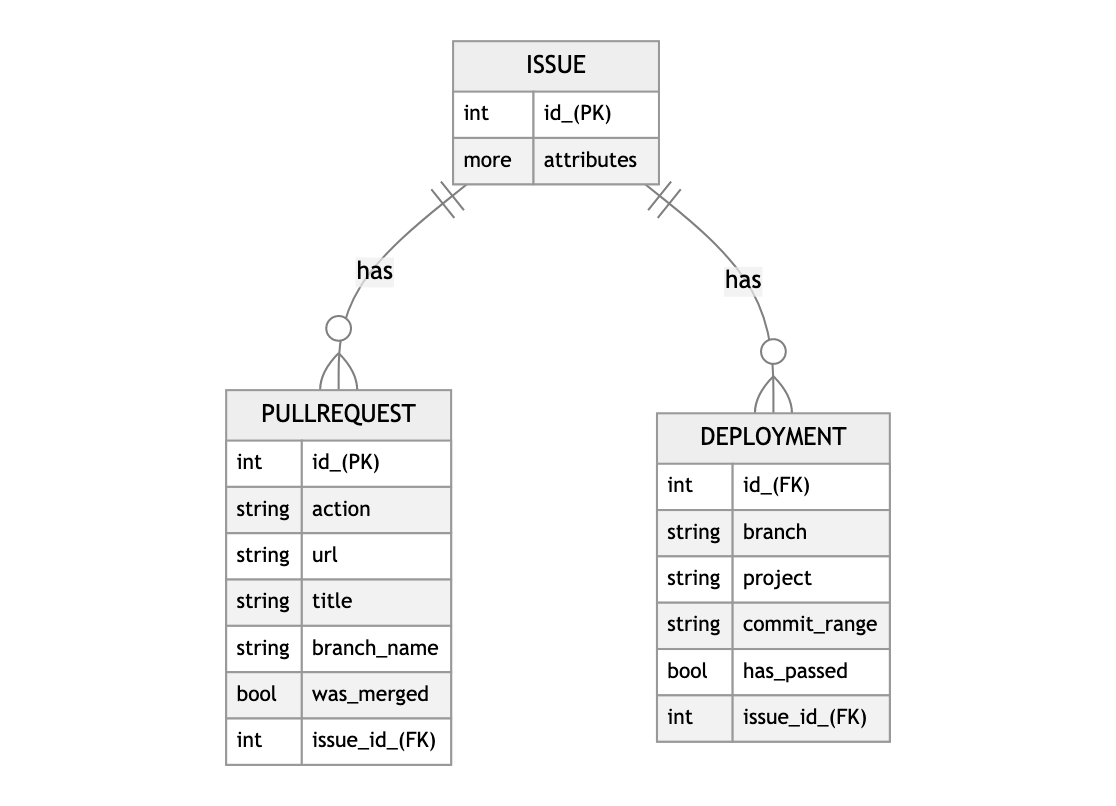
\includegraphics[width=0.8\textwidth]{images/erd/multiple.png}
  \label{fig:erd_multiple}
\end{center}

\subsubsection{Option 2: Inheritance}
Die zweite Option ist, dass für Deployments und Pull-Requests keine eigenen Entitäten erstellt werden, sondern diese von
einer gemeinsamen Entität erben. Das würde wie folgt aussehen:
\begin{center}
  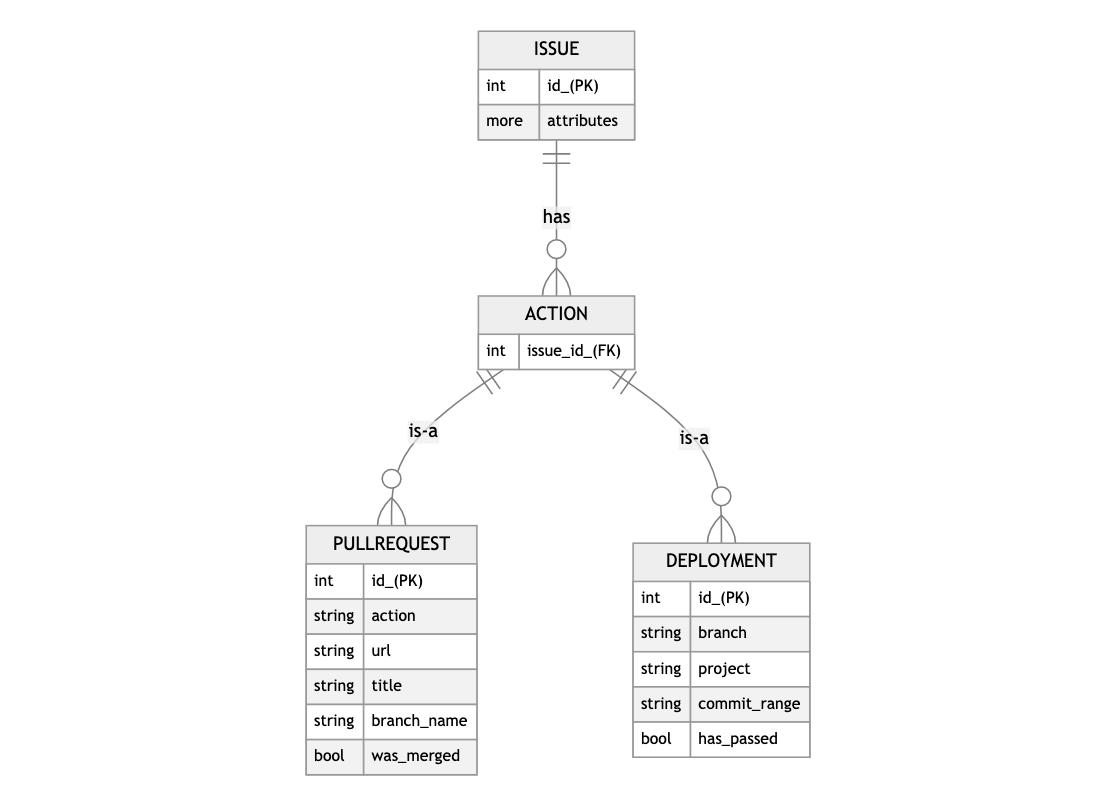
\includegraphics[width=0.8\textwidth]{images/erd/inheritance.png}
  \label{fig:erd_inheritance}
\end{center}

\subsubsection{Option 3: Has many through}
Die dritte Option ist, dass Deployments mit einer \enquote{has-many} Beziehung mit Pull-Requests verbunden werden. In diesem Fall hätte jedes
Issue mehrere Deployments \enquote{durch} die Pull-Requests. Daher der Name. Das würde wie folgt aussehen:
\begin{center}
  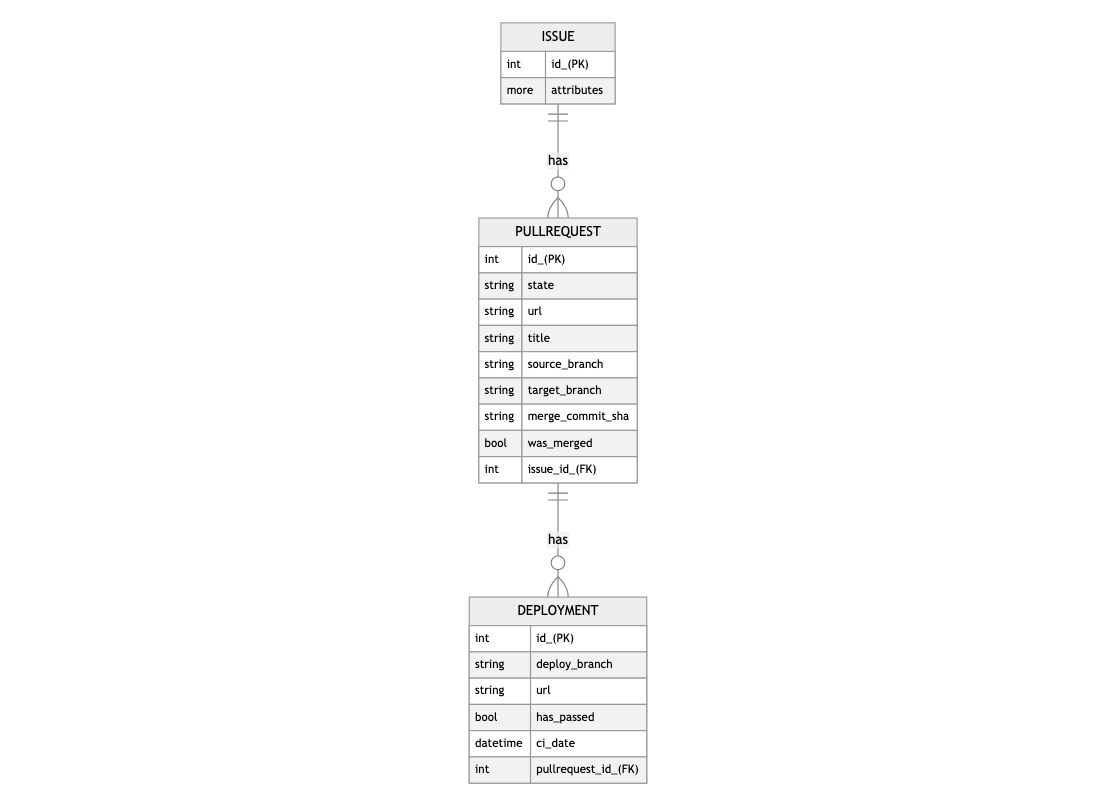
\includegraphics[width=0.8\textwidth]{images/erd/has_many_through.png}
  \label{fig:erd_has_many_through}
\end{center}

\subsection{Activity-Diagram}
\label{sec:activity_diagram}
Das Activity-Diagramm zeigt den Ablauf des Plugins. In diesem Fall gibt es zwei Abläufe:
\begin{itemize}
  \item Hook von SemaphoreCI oder GitHub
  \item Abfragen der Issues \newline
\end{itemize}

\subsubsection{Hook call}
Die Hook calls werden von SemaphoreCI oder GitHub ausgelöst. Beide bei unterschiedlichen Events, welche beide mit Sanduhren
dargestellt wurden:
\begin{center}
  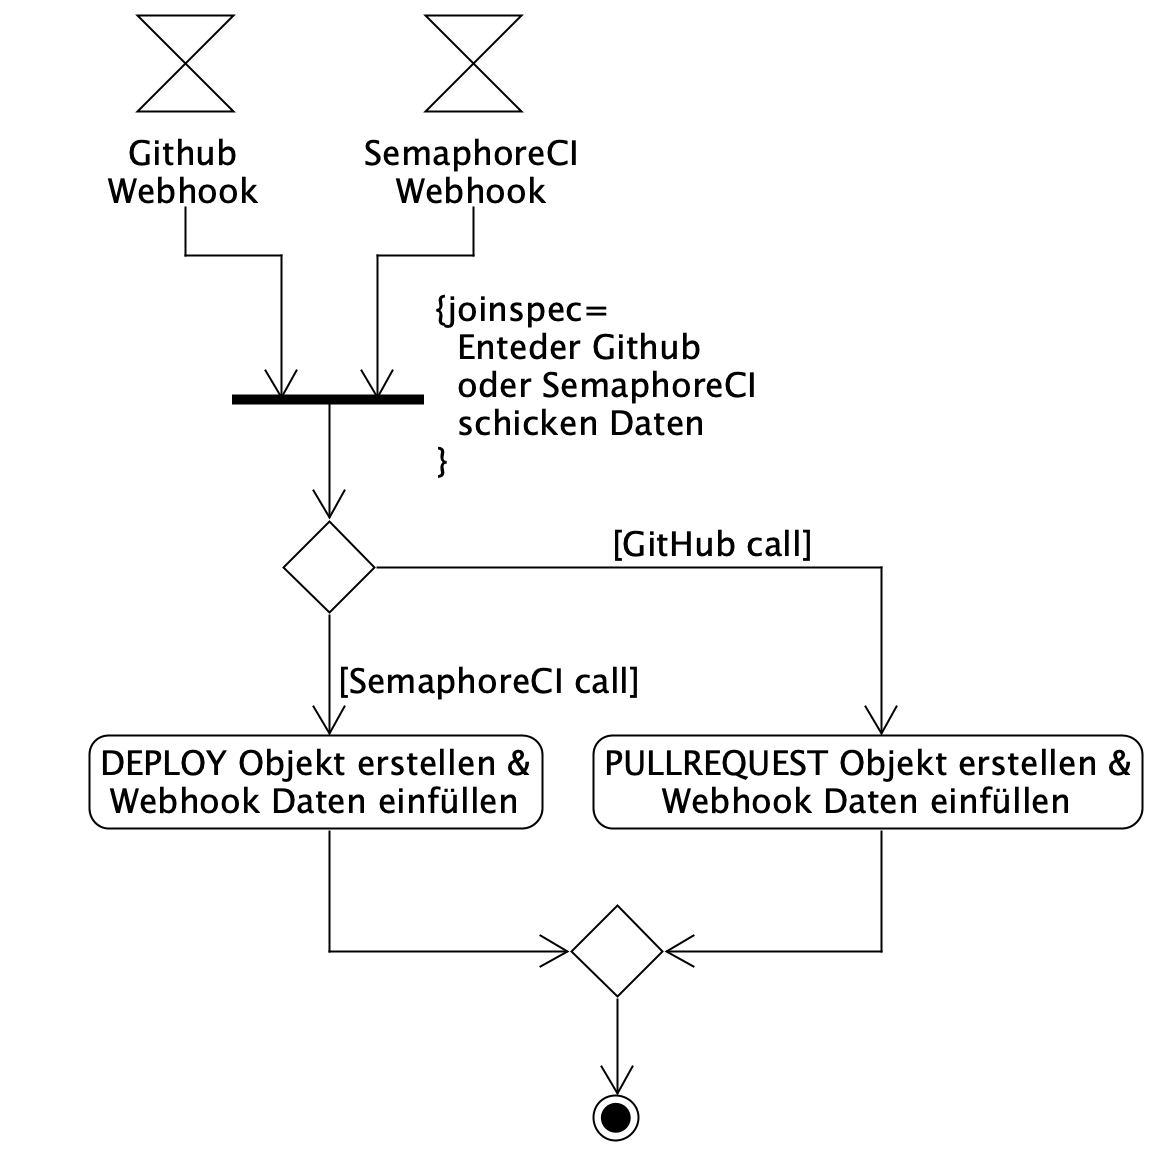
\includegraphics[width=0.8\textwidth]{images/activity/webhook.png}
  \label{fig:activity_hook_call}
\end{center}

\subsubsection{SemaphoreCI Plan B}
Da SemaphoreCI in den Webhook Daten nicht alle Commit-Hashes, sondern nur eine Range mitliefert, kann es sein, dass die
Informationen über welche Commits Deployed wurden, nicht vorhanden sind. Deswegen wird hier ein zweiter Vorschlag für den
SemaphoreCI Workflow präsentiert. Dieser würde direkt auf GitHub nachfragen wie die Commit-Geschichte aussieht. So
ungefähr würde das aussehen: \newline
\begin{center}
  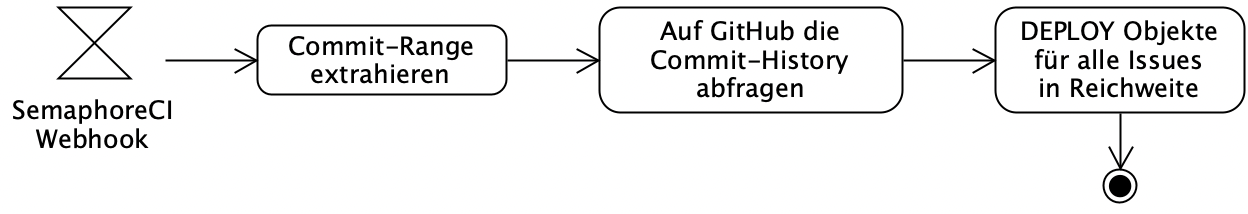
\includegraphics[width=0.8\textwidth]{images/activity/semaphore-backup-hooks.png}
  \label{fig:activity_plan_b}
  \newline
\end{center}
Falls diese Option implementiert wird, ändert sich das Deployment Diagramm ganz leicht, da jetzt
eine neue Brücke vom Plugin zu GitHub existiert. In rot markiert ist die neue Brücke: \newline
\begin{center}
  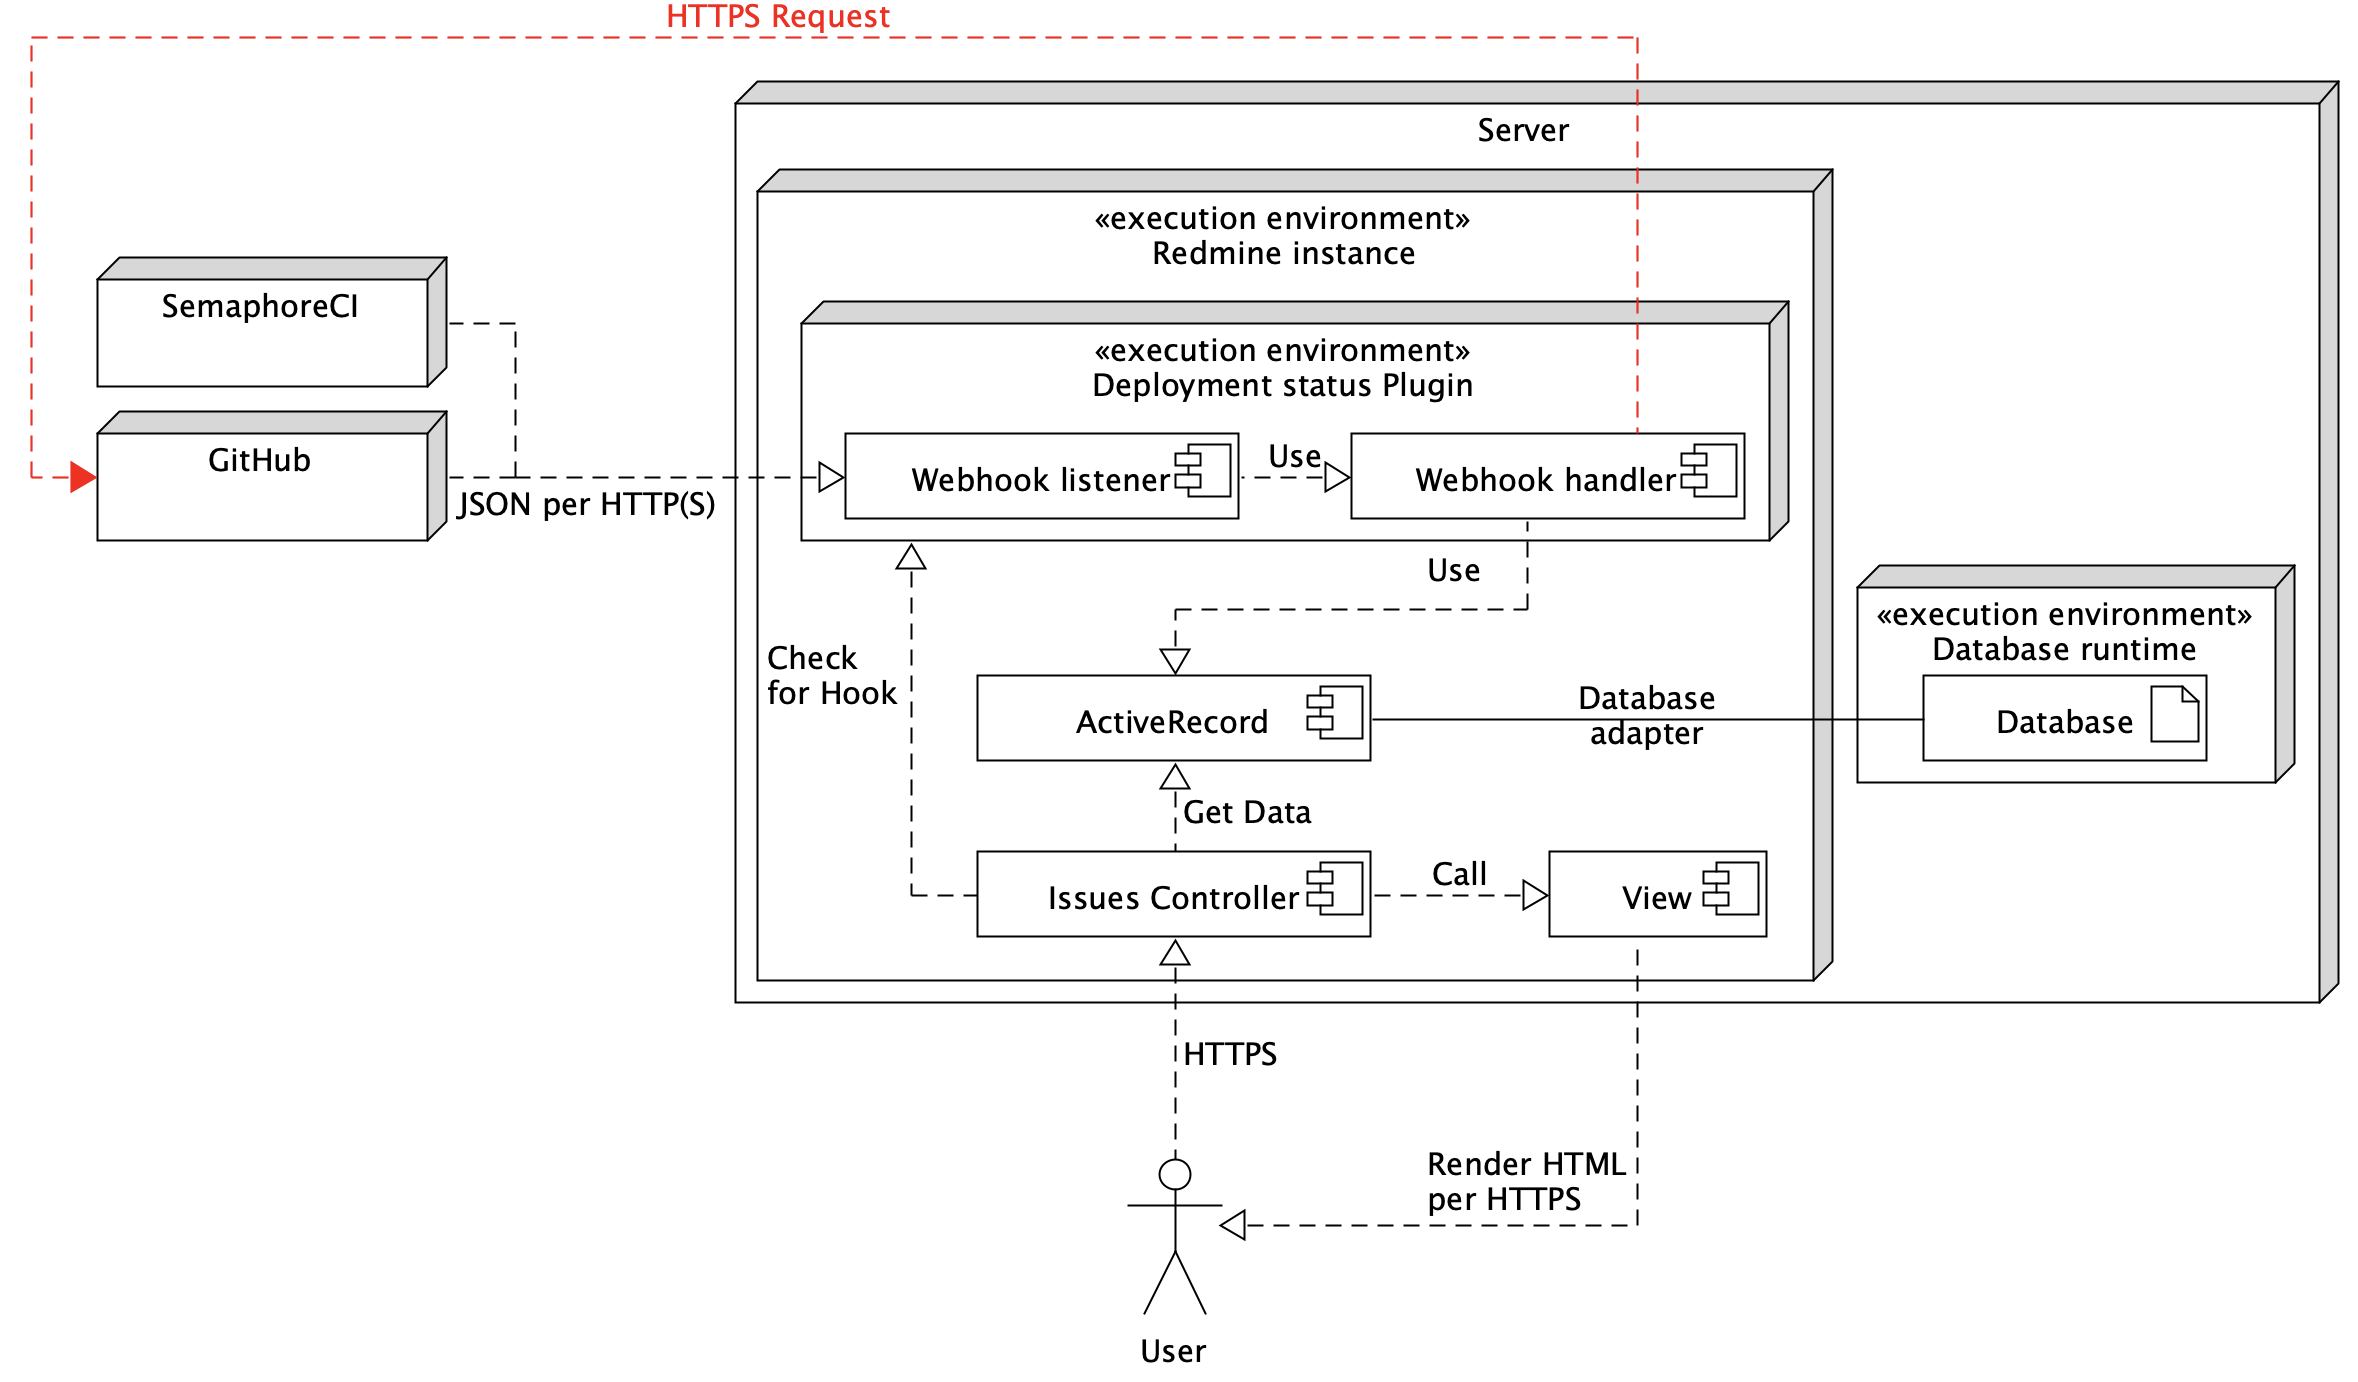
\includegraphics[width=0.8\textwidth]{images/deployment/backup-hooks.png}
  \label{fig:activity_plan_b_deployment}
\end{center}

\subsubsection{Abfrage der Issues}
Falls der Nutzer auf die Details eines Issues klickt, wird eine Abfrage an das Plugin gesendet, welches die Pull Requests sowie
Deployments abfragt und diese zurückgibt: \newline
\begin{center}
  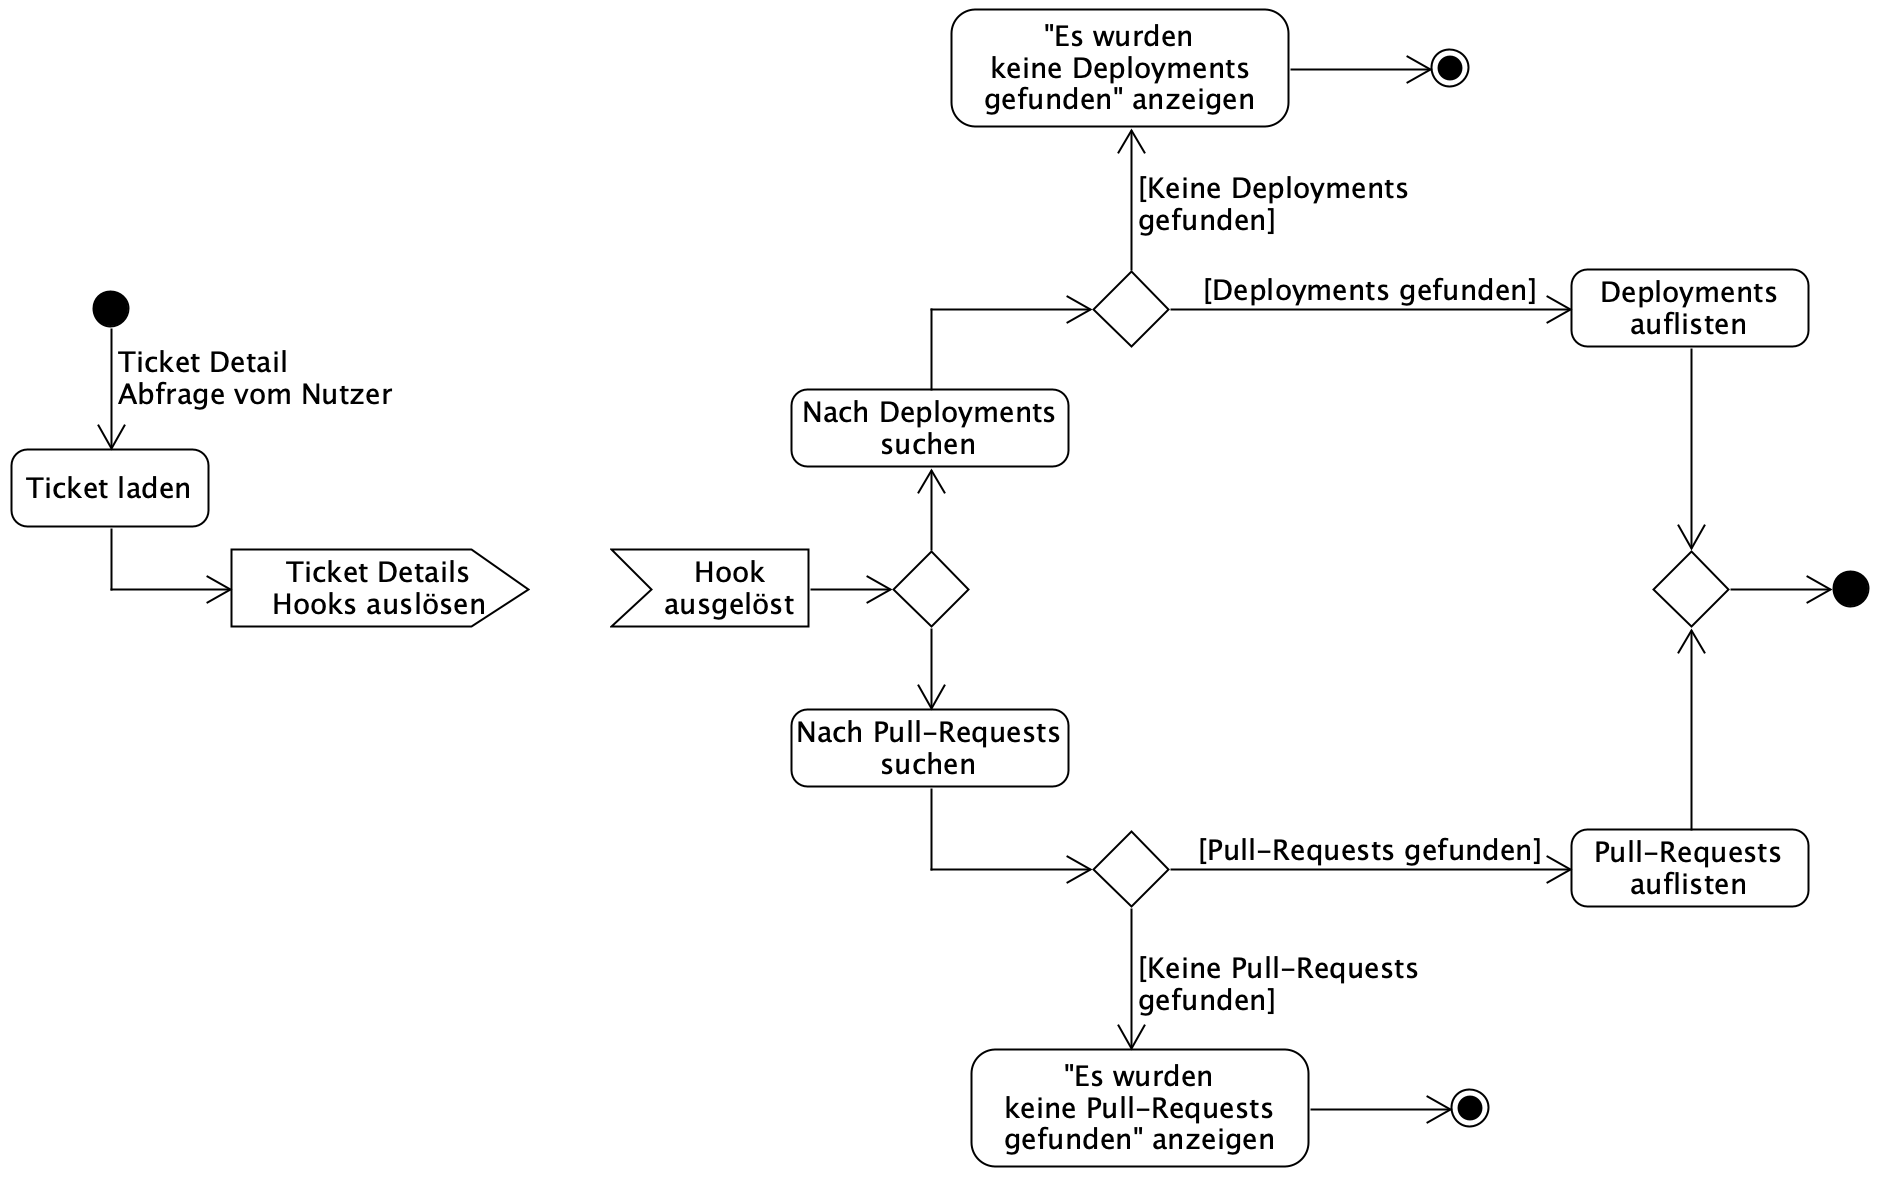
\includegraphics[width=0.8\textwidth]{images/activity/issues-view.png}
  \label{fig:activity_issues}
\end{center}

\subsection{Mockups}
\label{sec:mockups}
Damit die UI besser geplant werden kann, wird diese mit Mockups visualisiert. Diese Mockups sollen
nur ungefähr wiedergeben, wie die UI aussehen soll. Da das Plugin auf einer bereits existierenden 
Ansicht aufbaut, nämlich der Issue-View, wird diese nur sehr abstrahiert dargestellt. \newline
Die bereits existierende Ansicht ist in der Abbildung mit weniger Opazität dargestellt. \newline

  \subsubsection{Zwei Listen}
  Option eins ist, dass die Pull-Requests und Deployments in zwei Listen dargestellt werden. Das würde ungefähr so
  aussehen: \newline
  \begin{center}
    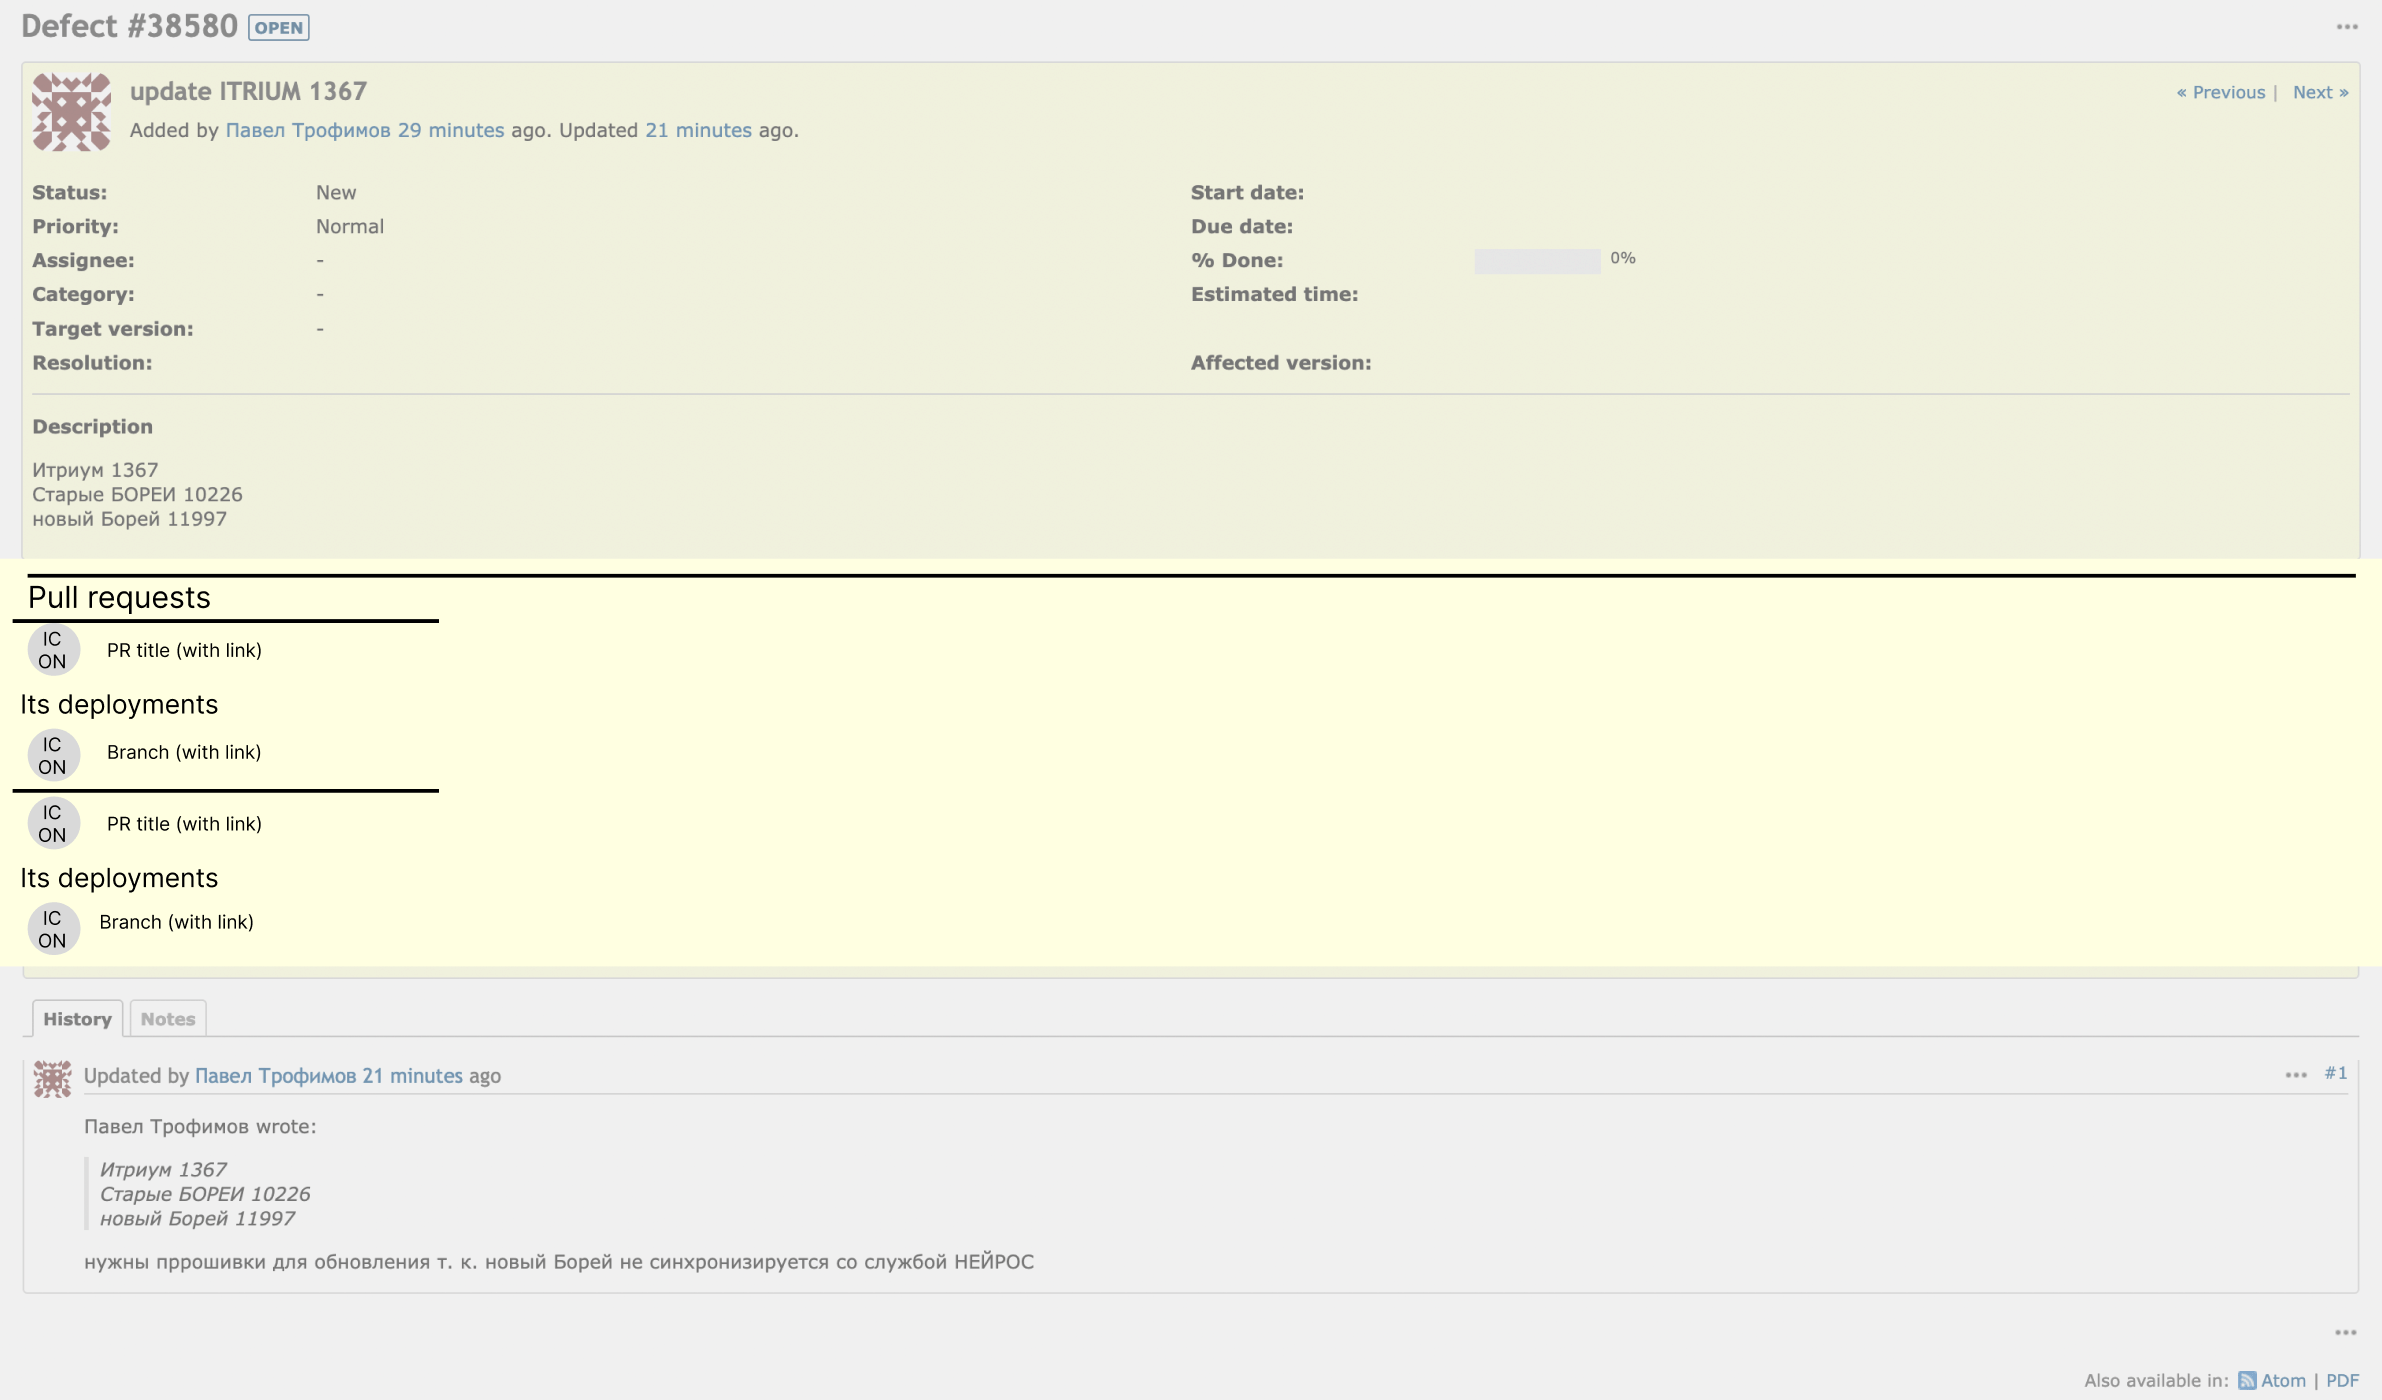
\includegraphics[width=0.8\textwidth]{images/mockup/multiple-lists.png}
    \label{fig:mockup_multi_lists}
    \newline
  \end{center}

  \subsubsection{Eine Liste mit Unterlisten}
  Die zweite Option ist, dass die Pull Requests aufgelistet werden und die Deployments als Unterlisten aufgelistet
  werden. So würde das aussehen: \newline
  \begin{center}
    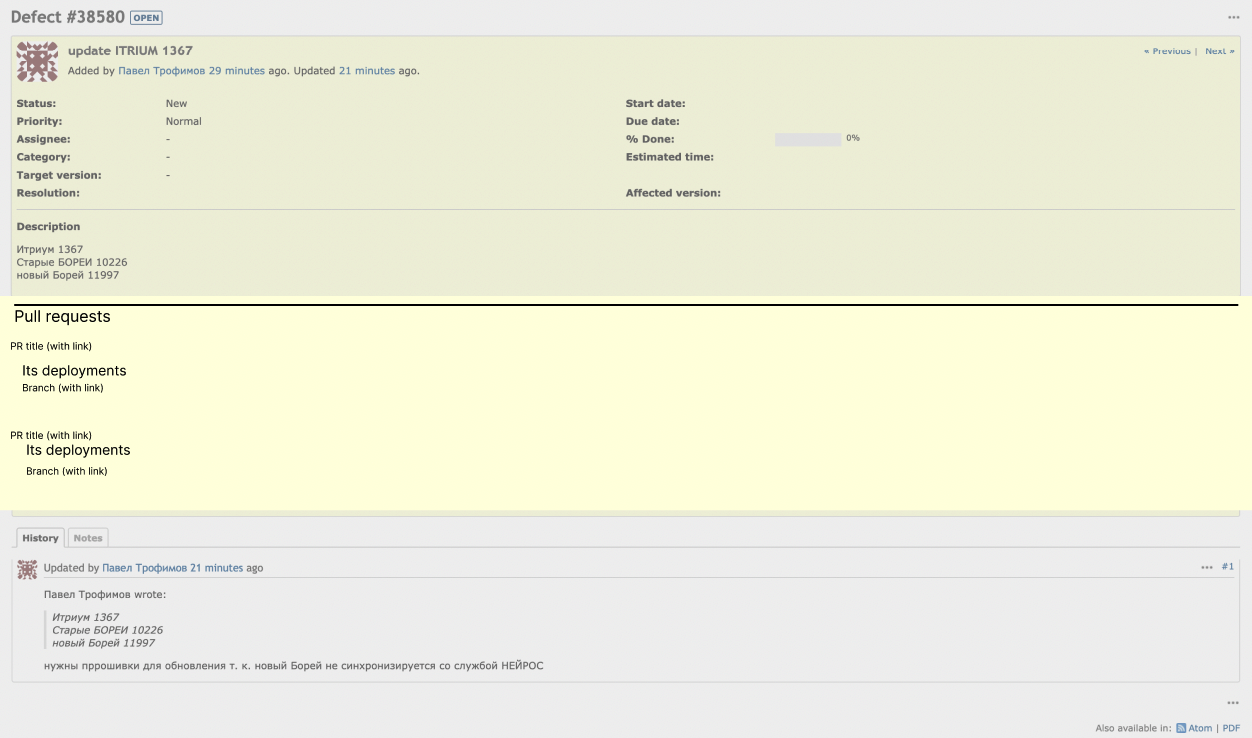
\includegraphics[width=0.8\textwidth]{images/mockup/sublists.png}
    \label{fig:mockup_sublists}
  \end{center}

\section{Testkonzept}
\label{sec:testkonzept}
Das Testkonzept beschreibt, wie und mit welchen Werkzeugen das Resultat auf seine Richtigkeit kontrolliert wird.

\subsection{Automatisierte Tests}
Es werden automatisierte Tests für das Plugin geschrieben, welche die Funktionalität der Applikation testen.
Diese werden mit den gleichen Frameworks wie die vom Redmine geschrieben. Das heisst, dass die Tests mit
folgenden Frameworks geschrieben werden:
\begin{itemize}
  \item \textbf{MiniTest} für die Unit-Tests
  \item \textbf{Capybara} für die System-Tests
\end{itemize}
Die coverage sollte 100\% betragen (bei Klassen über 5 Zeilen). Diese Tests werden dann automatisch auf 
SemaphoreCI ausgeführt. Von der CI erhalten wir dann einen Coverage-Report, sowie eine Liste der
fehlgeschlagenen Tests. Nur falls alles in Ordnung ist, kann man die Pull-Request mergen.

\subsubsection{Weitere Tools}
Tools, welche nicht von Redmine selbst verwendet werden, welche aber dennoch im Plugin verwendet werden sind:
\begin{itemize}
  \item \textbf{Faker} für das Erstellen von realistischen Testdaten.
  \item \textbf{FactoryBot} für das Initialisieren von Objekten.
\end{itemize}
Die Coverage, sowie andere wichtige Informationen werden unter \ref{sec:automated-tests} dokumentiert.

\subsection{Manuelle Tests}
Während der Entwicklung und für allfällige Demonstrationszwecke werden manuelle Tests durchgeführt. Diese
werden in diesem Kapitel beschrieben und unter \ref{sec:manual-tests} protokolliert.

\subsubsection{Allgemeiner Vorgang}
\label{sec:general-testing}
Um die Funktionalität des Plugins zu testen, muss eine eintreffende Webhook von SemaphoreCI oder GitHub simuliert werden.
Dabei hat man zwei Optionen:
\begin{itemize}
  \item \st{Senden von Daten per HTTP-Request an den lokalen Server}
  \item Benützen des Dienstes, damit dieser die Daten schickt
\end{itemize}

\textbf{Senden von Daten per HTTP-Request an den lokalen Server} \\
Option eins ist das manuelle Senden von Daten an den lokalen Server. Dies kann man in der Konsole mit dem curl Programm
\cite{everything_curl} machen. Dies ist jedoch eine sehr aufwändige und ungenaue Art zu testen, weshalb diese Option nicht
weiter verfolgt wird. \newline

\textbf{Benützen des Dienstes, damit dieser die Daten schickt} \\
Die zweite Option ist, ein Repository auf GitHub zu erstellen und dieses mit SemaphoreCI / Github Webhooks zu
verbinden. \newline
Damit dann diese Daten beim lokalen Server ankommen können, müsste man mit ngrok \cite{ngrok_http_docs} einen HTTP Tunnel
erstellen, welcher eine öffentliche IP zur Verfügung stellt. \newline
Diese Methode ist auch sehr aufwändig, doch liefert genauere Daten als Option eins, weshalb diese benutzt wird. \newline

\subsubsection{Verarbeiten von SemaphoreCI Daten}
Da unter Kapitel \ref{sec:general-testing} etabliert wurde, dass die Dienste wirklich verwendet werden beim manuellen Testen,
wird der Test nach folgenden Schritten durchgeführt:
\begin{enumerate}
  \item Ein Issue auf Redmine erstellen
  \item Auf GitHub ein Repository erstellen und dieses mit SemaphoreCI verbinden. 
  (\textbf{Wichtig:} Es muss ein Deploy-Skript erstellt werden. Dieses heisst wie folgt:
  [branchname]-deploy.sh)
  \item Eine Pull Request erstellen und mergen.
  \item Warten, bis die Pipeline auf SemaphoreCI durchgelaufen ist
  \item Auf dem Issue kontrollieren, ob die Daten korrekt angezeigt werden
\end{enumerate}

\textbf{Das zu erwartende Resultat ist,} dass in der Beschreibung des Issues ein Deployment angezeigt wird. Das kann entweder grün oder rot
sein, je nachdem ob die Pipeline erfolgreich durchgelaufen ist oder nicht.

\subsubsection{Verarbeiten von GitHub Daten}
\label{sec:github-testing}
Das Testen von den GitHub Webhooks lauft sehr ähnlich ab:
\begin{enumerate}
  \item Ein Issue auf Redmine erstellen
  \item Auf GitHub ein Repository erstellen
  \item Eine GitHub Webhook erstellen, welche bei PRs Daten schickt. (Die URL muss auf den lokalen Server zeigen)
  \item Einen feature Branch erstellen (\textbf{Wichtig:} Die Issue-Nummer muss im Branchnamen enthalten sein)
  \item Eine Pull Request erstellen
  \item Auf dem Issue kontrollieren, ob die Daten korrekt angezeigt werden
\end{enumerate}

\textbf{Das zu erwartende Resultat ist,} dass in der Beschreibung des Issues eine Pull Request angezeigt wird. Da diese noch nicht gemerged
wurde, sollte es sichtbar sein, dass die Pull Request offen ist.

\subsubsection{Der Nutzer schaut sich ein Issue an mit Daten}
Für diesen Testfall wird auf einer lokalen Redmine Instanz ein Issue erstellt. Daraufhin werden die Schritte aus
\ref{sec:github-testing} durchgeführt, damit das Issue mit Daten vom Plugin befüllt wird. \newline
\textbf{Das zu erwartende Resultat ist,} dass die offene Pull Request angezeigt wird. Das sollte ohne grosse Ladezeit passieren, wie von 
Software-Design Anforderung drei verlangt.

\subsubsection{Der Nutzer schaut sich ein Issue an ohne Daten}
Für diesen Testfall wird einfach auf einer lokalen Redmine Instanz ein Issue erstellt. Dann wird in der Beschreibung des Tickets
kontrolliert, was angezeigt wird. \newline
\textbf{Das zu erwartende Resultat ist,} dass keine Daten angezeigt werden.

\subsection{Testmittel}
Als Testmittel werden folgende Tools verwendet:
\begin{itemize}
  \item \textbf{Redmine} für das Erstellen von Issues
  \item \textbf{GitHub} für das Erstellen von Repositories und Pull Requests
  \item \textbf{SemaphoreCI} für das Erstellen von Pipelines
  \item \textbf{ngrok} für das Erstellen von HTTP Tunnels
\end{itemize}
